\chapter{Implementacja}
W poniższym rozdziale opisane zostały prace nad modułem, przyczyny oraz uzasadnienie poszczególnych decyzji projektowych oraz problemów, które po drodze wyniknęły. Finalna architektura wraz z pełnym wyjaśnieniem funkcjonalności poszczególnych komponentów została opisana w rozdziale \ref{chapter_System_Architecture}.

\section{Podstawowy projekt zapoznawczy}
Pierwszym krokiem w utworzeniu modułu było utworzenie aplikacji testowej. Używa ona tych samych bibliotek oraz API co końcowy moduł, ale w formie okrojonej, nie realizując założeń architektury systemu, a jedynie MVP - Minimal Viable Product. Takie rozwiązanie pozwala na zapoznanie się z praktycznym wykorzystaniem używanych później interfejsów, a także na stworzenie wzorca do pierwszej implementacji faktycznego modułu docelowego.

Prace nad aplikacją rozpoczęto od utworzenia rozwiązania w programie Visual Studio 2022 na podstawie załączonego do niego wzorca - \textit{Direct3D 11 Game Win32} \cite{GitHub:walbourn:directx-vs-templates}, zawierającego prekonfigurowany projekt wykorzystujący Direct3D oraz DirectXTK. W ramach szablonu zawarte są też podstawowe metody tworzenia zasobów używanych w ramach D3D, a także przyjęta przez jej autora struktura sterowania przepływu kodu - inna od zaplanowanej w ramach modułu. Następnie dodane zostały zgodne z założeniami biblioteki i przetestowano poprawność konfiguracji. Do tak skonfigurowanego projektu dodane zostały metody wczytywania geometrii podstawowych modeli za pomocą biblioteki assimp, a także bez określonej struktury kod odpowiedzialny za ich dodatkową obróbkę oraz finalne renderowanie.  Projekt aplikacji zapoznawczej został zakończony implementacją widoku z obracającym się, kolorowym trójkątem. 

% TODO: Screenshot przedstawiający projekt zapoznawczy.

\section{Moduł rdzeniowy}
Tak przygotowany projekt umożliwiał względnie proste utworzenie aplikacji renderującej wczytany z dysku model, ale ze względu na brak konkretnej architektury oraz celu nie nadawał się do dalszego rozwoju. Kolejnym krokiem było więc przeniesienie już istniejących funkcjonalności do formy zgodnej z docelową architekturą, możliwą do dalszego rozwoju. W tym celu utworzona została podstawowa struktura \textbf{D3DEngine} (przemianowana później na \textbf{D3DCore}), przechowująca referencje do rdzeniowych zasobów systemu Direct3D oraz okna, a także odpowiedzialna za tworzenie, odpowiednie zarządzanie, użyczanie i zwalnianie tych zasobów. W kolejnym kroku do klasy dodane zostały nadpisywalne obiekty wskaźników na funkcje zdarzeń, wywoływanych przy niektórych interakcjach użytkownika z oknem - takich jak jego przesunięcie, zmiana rozmiaru czy aktywnego okna. Poprawiona została także wydajność ze względu na przejście ze starego trybu publikacji klatek obrazu - DXGI\_SWAP\_EFFECT\_BLIT - na nowy - DXGI\_SWAP\_EFFECT\_FLIP. 

\subsection{Wiele okien - wiele problemów}
W tym momencie zapadła decyzja, według której powinna być możliwość niezależnego działania wielu instancji modułu jednocześnie, co pozwoliłoby na utworzenie aplikacji klienta z funkcjonalnością otwierania wielu okien w ramach jednej aplikacji. Z takim podejściem wiąże się natomiast problem - WinAPI posiada możliwość zdefiniowania funkcji odpowiadającej na event zdarzeń okna \textit{(WndProc)}, ale bez bezpośredniej możliwości powiązania uchwytu okna do własnej struktury go reprezentującej. Po wielu testach różnych rozwiązań ostatecznie problem został rozwiązany pewnym obejściem. Przy tworzeniu okna wskaźnik na strukturę \textit{Window} zostaje przekazany jako ostatni argument funkcji CreateWindowEx - \textit{(lpParam)}. Następnie między WinAPI, a faktycznym eventem WndProc dodany zostaje pośrednik - WndProcDispatcher. Nasłuchuje on konkretnych typów zdarzeń i jeśli otrzyma event typu \textit{WM\_NCCREATE}, oznaczający utworzenie nowego okna, pobiera wskaźnik do struktury \textit{Window} przekazany jako pole struktury \textit{LPCREATESTRUCT} w argumencie lParam. Następnie wykonuje powiązanie z uchwytem do okna przy pomocy mechanizmu \textit{SetWindowLongPtr()}. Dzięki takiemu podejściu w kolejnych wywołaniach \textit{WndProcDispatcher} możliwe jest pobranie wskaźnika do powiązanej z uchwytem struktury przy pomocy funkcji \textit{GetWindowLongPtr()}, a w związku z tym wywołanie metody \textit{WndProc} na odpowiednim oknie. Pseudokod realizujący opisany mechanizm został przedstawiony na listingu \ref{lst:module:WndProcDispatcher}.

\begin{lstlisting}[caption={Pseudokod integracji wskaźnika okna z uchwytem HWND}, label={lst:module:WndProcDispatcher}]
void Window::Create() {
 ...
 CreateWindowEx(..., this);
 ...
}

LRESULT WndProcDispatcher(HWND hwnd, UINT message, (...), LPARAM lParam) {
 if (message == WM_NCCREATE) {
     Window* win = (LPCREATESTRUCT)lParam -> lpCreateParams;
     SetWindowLongPtr(hwnd, GWLP_USERDATA, win);
 }
	
 Window* win = GetWindowLongPtr(hwnd, GWLP_USERDATA);
 return win->WndProc(...);
}
\end{lstlisting}

\subsection{Mesh i typy wierzchołków}
Kolejnym napotkanym problemem okazał się być temat typu wierzchołków w ramach modeli i mesh'y. Do poprawnego działania Direct3D wymaga określenia struktury danych wejściowych w ramach mechanizmu InputLayout, która zmienia się w zależności od użytej struktury opisującej typ wierzchołków. Oczywistym rozwiązaniem byłoby użycie mechanizmu szablonowania z języka C++, ale wymagałoby to ręcznego i zewnętrznego definiowania implementacji metody zwracającej D3DInputLayout dla każdego typu wierzchołka z osobna, co jest bardzo podatnym na błędy i nieprzejrzystym rozwiązaniem. Tutaj także udało się znaleźć lepsze rozwiązanie, którym okazał się być wprowadzony w ramach C++20 mechanizm \textit{concepts} \cite{cpp20:concepts:2025}. W ramach tego mechanizmu możliwe jest zdefiniowanie \textit{konceptu}, czyli ograniczeń dla typów szablonowych narzucających im konieczność zawarcia określonej metody. Dzięki temu utworzony został koncept \textit{VertexTypeConcept}, który wymaga utworzenia metody \textit{GetInputLayout()}, zwracającej D3DInputLayout przystosowany do pracy z danym typem.

\subsection{Lewoskrętny układ współrzędnych}
Przewijającym się przez cały proces developmentu - a w tym momencie po raz pierwszy - problemem był także przyjęty jako zalecany w ramach Direct3D lewoskrętny układ współrzędnych, w którym oś +Z rośne wraz z głębokością "w ekranie". Jest to przeciwieństwo układu prawoskrętnego z odwróconą osią Z, wykorzystywanego przez większość konkurencyjnych API, takich jak OpenGL i Vulkan. Większość otwarto-źródłowych bibliotek oraz dostępnej dokumentacji opiera się na drugiej opcji, co skutkowało okazjonalnymi problemami z mieszaniem skrętności układów współrzędnych. Assimp posiada flagę postprocessingu, mającą na celu zmianę układu na lewoskrętny - \textit{aiProcess\_ConvertToLeftHanded} - która pomogła na tym etapie, ale nie naprawiła problemu całkowicie, przez co problem będzie wracać.

% TODO: Render bez poprawnej konwersji skrętności.

\subsection{Właściwości materiałów - wczytywanie}
Dane właściwości materiałów, takie jak jego kolor, chropowatość i inne parametry są odczytywane i dekodowane przez assimp przy wczytywaniu plików modeli. Dane te zapisane są jednak w formie tablicy bajtów, niezależnie od tego jaki typ reprezentują. Wczytanie takich danych wiąże się z dwoma potencjalnymi trudnościami - endianness architektury oraz brak wsparcia dla operacji na bitach przy typach zmiennoprzecinkowych.

Pierwszy problem opisuje potencjalną niekompatybilność bitowego zapisu wielobajtowych danych dla różnych architektur. W przypadku systemów Big Endian, dane przechowywane są bajtami w kolejności od najbardziej do najmniej znaczącego, gdzie Little Endian sortuje je odwrotnie. Brak konwersji między typami spowodowałby niepoprawną interpretację danych, a w rezultacie błędne parametry wynikowe. Najważniejsze architektury na rynku są jednak zgodne - procesory ARM oraz x86 operują na założeniu Little Endian \cite{ARM:Developer:Endianness} \cite{Oracle:HelpCenter:x86ByteOrdering}. W związku z tym podjęta została decyzja, aby nie dodawać osobnej ścieżki kodu dla architektur Big Endian, ze względu na niską popularność takich systemów.

Druga trudność wynika ze standardu IEEE 754, opisującego standard typów zmiennoprzecinkowych \textit{(ang. floating point)}, na podstawie którego zaimplementowany został typ float w języku C++. Standard ten zabrania bezpośredniej manipulacji bitami, a także bezpośredniej konwersji bitowej z innych typów, a jedynie na konwersję wartości. Fakt ten nie pozwala na łatwe wczytanie zapisanych w formie tablicy bajtów liczb zmiennoprzecinkowych i wymaga obejścia, polegającego na konwersji wskaźnika na pointer typu float, a następnie pobranie jego wartości.  W taki sposób, przedstawiony na listingu \ref{lst:module:floatingPointHack}, możliwe jest wczytanie reprezentacji bitowej do formy natywnej zmiennej typu float.

\begin{lstlisting}[caption={Bitowa konwersja typu całkowitego na float w C++}, label={lst:module:floatingPointHack}]
// Wczytanie danych z tablicy bitów
int numberFromBytes = loadBytes();

// Wczytanie adresu do wskaźnika
int* nfbPointer = &numberFromBytes;

// Konwersja wskaźnika typu całkowitego na typ float
float* fprPointer = (float*)nfbPointer;

// Pobranie wartości z nowego wskaźnika.
float floatingPointRepresentation = *fprPointer;
\end{lstlisting}

\subsection{Właściwości materiałów - przechowywanie}
Po wczytaniu parametry materiału należy także przechować. Ze względu na specyfikę tych danych - a w szczególności różne typy danych zależnie od rodzaju parametru - pojawił się problem w jaki sposób powinno to zostać zrealizowane. Pierwotnie rozważane było użycie polimorfizmu ze wspólnego interfejsu, ale specyfika użycia wymagałaby każdorazowej konwersji na typ pochodny, co zmniejsza użyteczność takiego rozwiązania. W związku z tym zdecydowano się na użycie unii między typami przy pomocy mechanizmu \textit{union} oraz dodatkowej zmiennej przechowującej aktualnie przechowywany typ. Unia składała się z dynamicznie alokowanej tablicy dla wektorów typów liczbowych i std::string do tekstu. Odczyt odbywał się przy pomocy dedykowanych do tego metod, które przed zwróceniem danych sprawdzały poprawność żądania. 

Po dokładnych testach mechanizm ten nie okazał się jednak niezawodny, gdyż śledzenie stanu unii oraz odpowiedniej dealokacji i realokacji przy wszystkich przypadkach brzegowych okazało się niepraktyczne i podatne na błędy. Ze względu na to unia zastąpiona została przy pomocy obiektu typu std::variant ze standardu C++17 \cite{cpp17:variant:2025}. Jest on bezpieczniejszym zamiennikiem dla unii, posiadającym wbudowane wsparcie dla złożonych mechanizmów zarządzania obiektami i pamięcią ze standardów po C++11. Sposób odczytu danych pozostał niezmieniony.

\subsection{Odtworzenie funkcjonalności projektu zapoznawczego}
Na tym etapie przeniesione zostało już większość funkcjonalności z projektu zapoznawczego, więc możliwym było zupełne usunięcie zależności od oryginalnej klasy Game. Na koniec ponownie zaimplementowane zostało demo kręcącego się trójkąta z wykorzystaniem nowego API, co symbolizuje początek prac nad projektem warstwy silnika. Aby ułatwić dalszą pracę wydzielony został osobny projekt nazwany \textbf{TestApp}, pełniący funkcję aplikacji klienckiej.

% TODO: Demo trójkąta zrealizowane przy pomocy nowego systemu. 
% TODO: Porównanie złożoności implementacji interfejsów.

\section{Warstwa sceny}
Po ukończeniu warstwy rdzeniowej przyszła kolej na część sceny. Implementacja jej funkcjonalności rozpoczęła się od utworzenia bazowego obiektu sceny oraz struktury nimi zarządzającej - \textbf{Scene}. Następnie zaimplementowane zostały metody tworzenia, usuwania oraz przypisywania do hierarchii obiektów - odpowiednio \textit{Instantiate()}, \textit{Destroy()} i \textit{SetParent()}. Wzajemna hierarchia obiektów musiała zostać podparta strukturą zarządzającą ich wzajemnymi relacjami oraz transformacjami przestrzennymi, w związku z czym powstała odpowiedzialna za to klasa \textbf{Transform}, wykorzystująca macierze transformacji do odwzorowania wzajemnych relacji między obiektami.

\subsection{Gimbal Lock}
Jednym z częściej spotykanych problemów w reprezentacji transformacji jest rotacja. Jej intuicyjna implementacja w postaci wektora trzech elementów reprezentujących rotację w 3 osiach przestrzeni jest bowiem podatna na błąd zwany \textit{Gimbal Lock}. Jest to sytuacja, w której wraz z obrotem obiektu obraca się także układ współrzędnych wokół którego jest on obracany, a w rezultacie wykonanie tych samych rotacji w innej kolejności może doprowadzić do innej pozycji wynikowej, co zostało pokazane na rys. \ref{GimbalLock}.

Rozwiązaniem jest dodanie czwartego wymiaru o aktywnym balansie, określającego "niezależny" układ współrzędnych. Standardem realizacji tego konceptu jest struktura kwaternionów, która po dodaniu metod balansujących idealnie nadaje się do reprezentacji rotacji w przestrzeni trójwymiarowej. Do dalszej pracy użyta została implementacja \textit{Quaternion} zawarta w ramach pakietu SimpleMath.

\begin{figure}
	\centering
	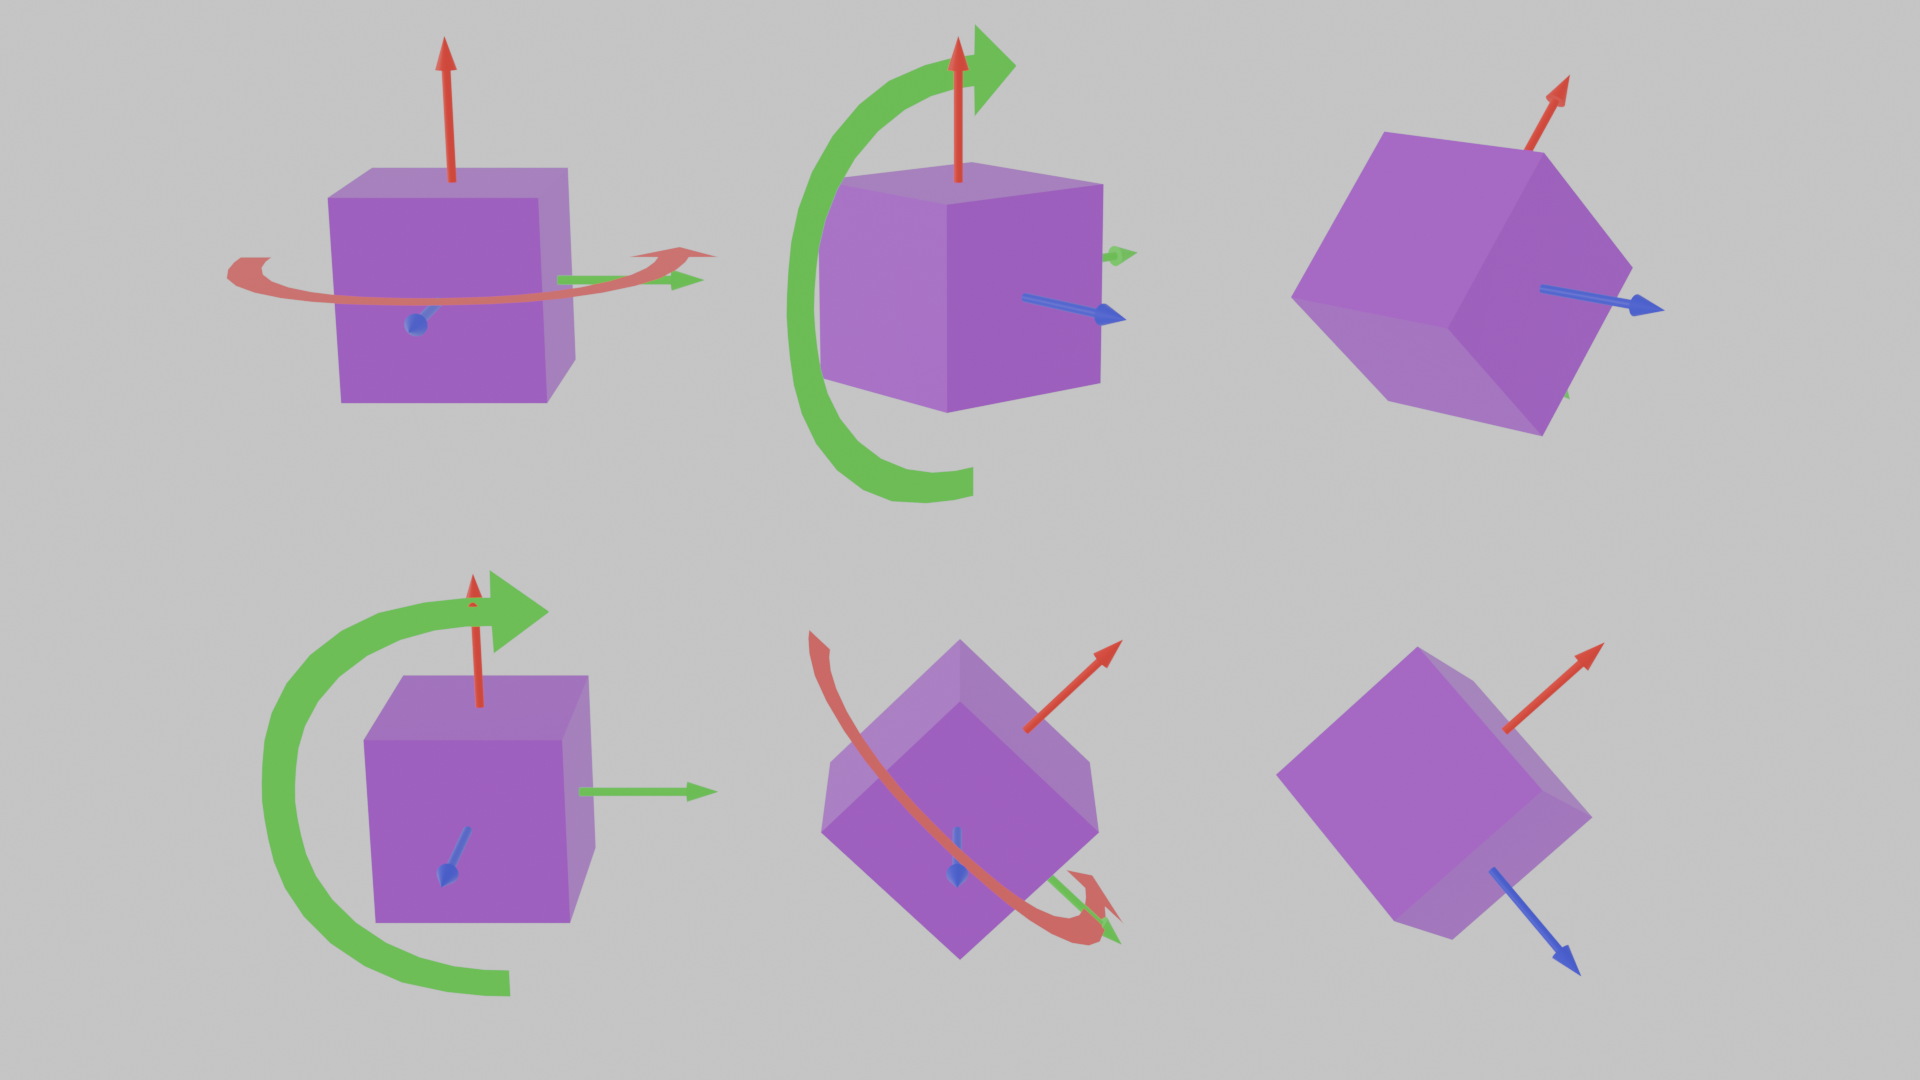
\includegraphics[width=\textwidth]{images/gimbal_lock.png}
	\caption{Wizualizacja efektu gimbal lock.}
	\label{GimbalLock}
\end{figure}

\subsection{Transformacje w przestrzeni}
Autor miał już doświadczenie w projektowaniu komponentów zbliżonych do \textit{Transform}, ale opierało się ono na API OpenGL i bibliotece GLM, zamiast użytego w projekcie Direct3D i DirectXTK / SimpleMath. Większość metod udało się utworzyć z małymi zmianami, ale problemem okazała się być metoda \textit{LookAt(target, upVector)}, która obraca obiekt w stronę przekazanej w ramach parametru \textit{target} docelowej pozycji w przestrzeni.  W pakiecie GLM znajduje się dedykowana do tego funkcja glm::lookAt() \cite{glm:docs:look_at}, której odpowiednika brakuje w pakiecie DirectXTK, więc funkcjonalność musiała zostać odtworzona. 

Pierwszym podejściem była próba wykorzystania dostępnej w DXTK metody \textit{XMMatrixLookAtLH()}, tworzącej macierz transformacji odpowiadającą rotacji kamery patrzącej na odpowiedni punkt. Wynikową macierz należy następnie odwrócić, aby przekonwertować ją na wersję dla obiektu i na jej podstawie utworzyć kwaternion rotacji. 